\chapter{Fundamentos do Método \MT}
    \label{cap-fundamentosMT}    
    
    O método \MT proposto por \citeauthor{tikhonov50} \citeyearpar{tikhonov50} e
    \citeauthor{cagniard53} \citeyearpar{cagniard53}, usa as propriedades
    eletromagnéticas para estudar a distribuição de resistividade elétrica na crosta, 
    podendo variar a sua investigação de dezenas de metros a dezenas de 
    quilômetros.
    
    \section{Origem das Correntes Telúricas}
    
    As flutuações no campo magnético terrestre geram campos elétricos na alta atmosfera que induzem correntes magnéticas.
    
    As ondas eletromagnéticas penetram no interior da Terra na forma de ondas planas ortogonais que induzem novas correntes chamadas de corrente telúricas que trazem informações das características físicas das litologias \cite{tikhonov50} e \cite{cagniard53}.
    
    Uma das características é a modulação da frequência, causada por diferentes tipos de rochas e estruturas, esse fenômeno é diretamente 
	relacionado a resistividade elétrica do meio. As frequências das ondas são baixas variando de 1 $mHz$ à 10 $kHz$.
	
	Ondas com frequências menores que 1 $Hz$ tem origem nos ventos solares que interagem com o campo magnético terrestre, já ondas com frequências maiores de 1 $Hz$ são provocadas por tempestades equatoriais. Para o estudo do \MT são feitas as seguintes suposições:
    
    \begin{enumerate}
	    \item Ondas geradas na ionosfera, distantes o suficientes, penetram ortogonais à superfície da Terra.	    
	    \item A Terra se comporta como um condutor ôhmico.
	    \item A Terra é considerada um semi-espaço isotrópico.
	\end{enumerate}   
    
    
%RESISTIVIDADE ==============================================================================================================================================
    \section{Resistividade dos Materiais}
    
    Para o \MT a propriedade de investigação e contraste é a condutividade elétrica ($\sigma$) ou resistividade elétrica ($\rho$) sendo essa o inverso da primeira.
    A resistividade elétrica é uma propriedade particular de um determinado material, ou seja, a partir de uma resistividade elétrica podemos estimar a qual material ela pertence\footnote{Para os meios geológicos essa propriedade é representada por um intervalo de valores, devido as complexidades químicas e físicas das diferentes litologias.}.
    
    Em 1827, Georg Ohm verificou de forma empírica que aplicando uma diferença de potencial em um material, esse gera uma resistência à passagem de corrente, essa relação é chamada de lei de Ohm (equação \ref{lei_de_ohm}) \cite{eletromag8hayt}.
    
    \begin{equation}
        \label{lei_de_ohm}
        V = R i
    \end{equation}
    
    Onde $V$ é a diferença de potencial (Volts - V), $i$ é a corrente (Ampère - A) e $R$ é a resistência (Ohms - $\Omega$), materiais que obedecem essa lei são chamados de materiais ômicos.
    
    A Terra pode ser considerada como um material ôhmico. No entanto para a investigação geofísica a resistência não é uma propriedade viável, visto  que depende muito da geometria do problema, assim foi proposto a resistividade elétrica, onde, um mesmo material terá a sua resistividade elétrica igual, independente da geometria.
    
    A figura \ref{fig_resistividade} mostra um circuito para se obter a resistividade elétrica de um material, sendo A a área [$m^2$], R a resistência [$\Omega$], L o comprimento [$m$] e $\rho$ a resistividade elétrica dada em $\Omega m$. 
    
    \begin{equation}
        \label{resistividade}
        \rho = \dfrac{R A}{L}\, \, \, ;\, \, \, \, \, \, \, \, \, \, \, \, \, \,  R = \dfrac{V}{i}
    \end{equation}
    
    
    \begin{figure}[h]
        \centering
        \caption{Arranjo para medir a resistividade elétrica ($\rho$) de um material}
        \centerline{\includegraphics[width=4cm]{texto/fig/resisti_telford.png}}
        \fonte{Adaptado \citeauthor{telford}, \citeyearpar{telford}}
        \label{fig_resistividade}
    \end{figure}
    
    A figura \ref{tabela_resistividade} mostra a distribuição de resistividade elétrica para diversos materiais geológicos. 
    Portanto podemos identificar a partir de um contexto geológico quais litologias pertencem a cada resistividade elétrica encontrada.
    
    Por exemplo, uma litologia que tenha resistividade elétrica em torno de  $100 \, \Omega m$ e outra com $3000 \, \Omega m $ pode ser caracterizada como um arenito e uma rocha ígnea respectivamente. 
    
    \begin{figure}[h]
        \centering
        \caption{Resistividade Elétrica dos Materiais Geológicos}
        \centerline{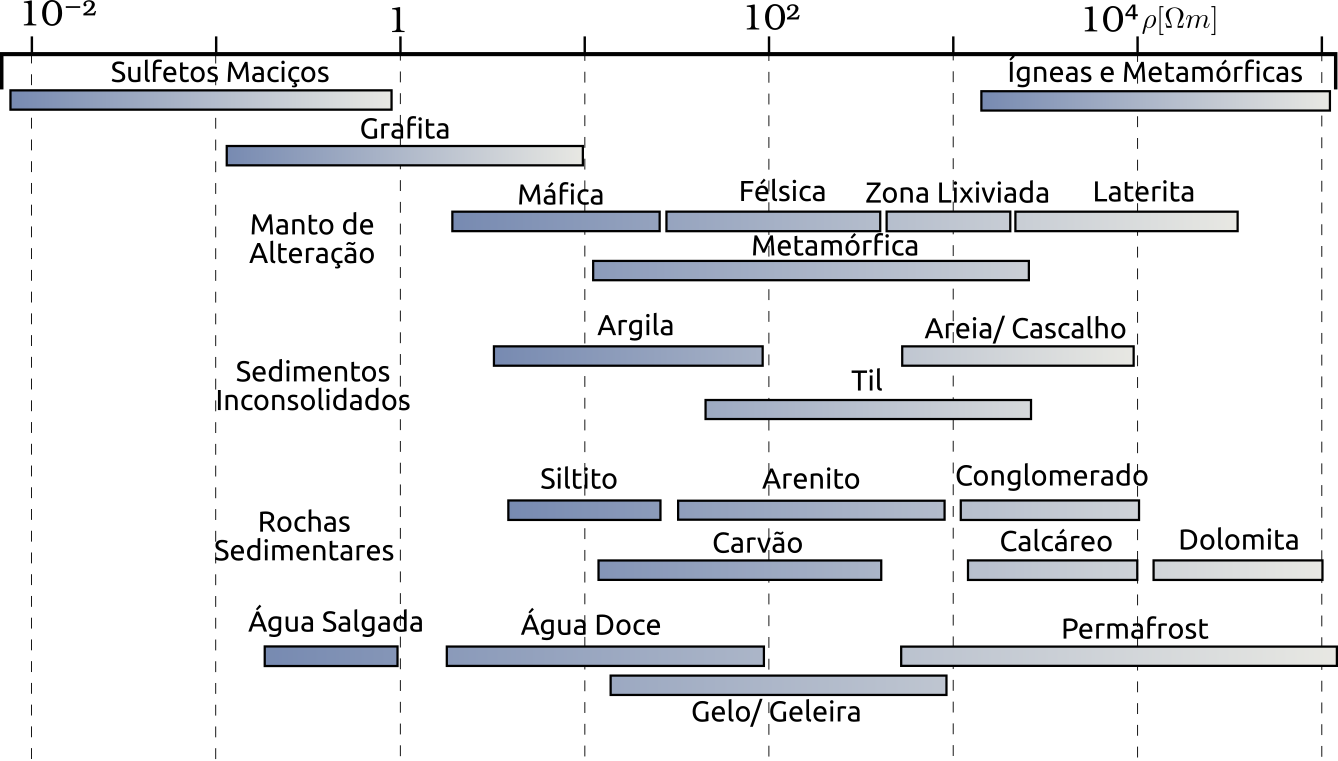
\includegraphics[width=14cm]{texto/fig/resistividade_tabela.png}}
        \fonte{Adaptado \citeauthor{eletromag_met}, \citeyearpar{eletromag_met}}
        \label{tabela_resistividade}
    \end{figure}
% FIM RESISTIVIDADE
%===========================================================================================================================================================    
    
    
    
% Eletromagneticos
%===================================================================================================================================================
    \section{Fundamentos Teóricos dos Métodos Eletromagnéticos}
        Usando as leis de Maxwell \cite{eletromag8hayt} podemos medir os campos elétricos e magnéticos e a partir deles estimar a resistividade elétrica dos meios litológicos em sub-superfície.
	
        Os campos podem ser descritos pelas seguintes equações\footnote{Para cargas e correntes livres
        (macroscópica)}:
            \begin{equation}
                \label{rot_elet_max}
                \nabla \times \vec{\textrm{E}}=-\frac{\partial \vec{\textrm{B}}}{\partial t} 
            \end{equation}
            \begin{equation}
                \label{rot_mag_max}
                \nabla \times \vec{\textrm{H}} = \vec{\textrm{J}} + \frac{\partial \vec{\textrm{D}}}{\partial t}
            \end{equation}
            \begin{equation}
                \nabla \cdot \vec{\textrm{B}} = 0
            \end{equation}
            \begin{equation}
                \label{div_d}
                \nabla \cdot \vec{\textrm{D}} = \rho_f
            \end{equation}
            
            \noindent Onde,
            
            {\footnotesize \noindent
            
            \begin{table}[H]
             \begin{tabular*}{1cm}{p{0.05cm}p{0.1cm}p{10cm}}
               {\footnotesize $\vec{\textrm{E}}$}  & {\footnotesize $\rightarrow$} & {\footnotesize Campo Elétrico [$V/m$] }\\
               {\footnotesize $\vec{\textrm{B}}$}  & {\footnotesize $\rightarrow$} & {\footnotesize Campo Magnético [$T$] }\\
               {\footnotesize $\vec{\textrm{H}}$}  & {\footnotesize $\rightarrow$} & {\footnotesize Campo Magnetizante [$A/m$]} \\
               {\footnotesize $\vec{\textrm{J}}$}  & {\footnotesize $\rightarrow$} & {\footnotesize Densidade de Corrente [$A/m^2$]} \\
               {\footnotesize $\vec{\textrm{D}}$}  & {\footnotesize $\rightarrow$} & {\footnotesize Campo de Deslocamento Elétrico [$C/m^2$]} \\
               {\footnotesize $\rho_f$}            & {\footnotesize $\rightarrow$} & {\footnotesize Densidade de Carga [$C/m^3$]} \\
               {\footnotesize $t$ }                & {\footnotesize $\rightarrow$} & {\footnotesize Tempo [$s$]}
             \end{tabular*}

            \end{table}}

            Obedecendo as relações de contorno para um meio isotrópico temos as seguintes
            relações (equações constitutivas):
            \begin{equation}
                \label{con_B}
                \vec{\textrm{B}} = \mu \vec{\textrm{H}}
            \end{equation}
            \begin{equation}
                \label{con_D}
                \vec{\textrm{D}} = \varepsilon  \vec{\textrm{E}}
            \end{equation}
            \begin{equation}
                \label{con_J}
                \vec{\textrm{J}} = \sigma \vec{\textrm{E}}
            \end{equation}
	    
	        {\footnotesize \noindent
            
            \begin{table}[H]
             \begin{tabular*}{1cm}{p{0.05cm}p{0.1cm}p{10cm}}
               {\footnotesize $\mu$}          & {\footnotesize $\rightarrow$} & {\footnotesize Permeabilidade Magnética [$H/m$] }\\
               {\footnotesize $\varepsilon$}  & {\footnotesize $\rightarrow$} & {\footnotesize Permissividade Elétrica [$F/m$] }\\
               {\footnotesize $\sigma$}       & {\footnotesize $\rightarrow$} & {\footnotesize Condutividade Elétrica [$S/m$]} \\
             \end{tabular*}

            \end{table}}
	    
	    
            Cada escalar das equações anteriores são características que dependem do meio em que a onda se propaga. Para a crosta $\mu = 1,2566\textrm{x}10^{-6} H/m$ e $\varepsilon = 8,85
            \textrm{x}10^{-12} F/m$; esses parâmetros funcionam como tensores em um meio
            anisotrópico que variam em função do tempo. Considerando para os 
            trabalhos de investigação o meio supõe-se ser isotrópico, assim, 
            tornando estáticos os tensores.
	
            Através das propriedades dos meios isotrópicos podemos reescrever as equações \ref{rot_elet_max} e \ref{rot_mag_max} usando as equações constitutivas \ref{con_B}, \ref{con_D} e \ref{con_J}.
            
            \begin{equation}
                \label{rot_elet_con}
                \rot{E} = - \mu \parct{H}
            \end{equation}
            
            \begin{equation}
                \label{rot_mag_con}
                \rot{H} = \sigma \ven{E} + \varepsilon \parct{E}
            \end{equation}
            
            Derivando a equação \ref{rot_mag_con} no tempo, multiplicando por $\mu$ e usando a equação \ref{rot_elet_con} temos:
            
            
\begin{align*}
\dfrac{\partial (\nabla \times \vec{\textrm{H}})}{\partial t} & = \dfrac{\partial (\sigma \ven{E})}{\partial t} + \dfrac{\partial}{\partial t} \bigg(\varepsilon \parct{E}\bigg)\\[10pt]
             \dfrac{\nabla \times \partial \ven{H}}{\partial t} & = \sigma \parct{E} + \varepsilon \parctto{E} \\[10pt]
             \mu \dfrac{\nabla \times \partial \ven{H}}{\partial t} & = \mu \sigma \parct{E} + \mu \varepsilon \parctto{E} \\[10pt]
             -\dfrac{\mu}{\mu} \nabla \times \rot{E} & = \mu \sigma \parct{E} + \mu \varepsilon \parctto{E}
             \end{align*}
             \begin{equation}
                \label{menos_rot_e}
              - \nabla \times \rot{E} = \mu \sigma \parct{E} + \mu \varepsilon \parctto{E}
             \end{equation}
                
            Usando a identidade vetorial:
            
            \begin{equation}
             \nabla \times \rot{A} = -\nabla^2 \ven{A} + \nabla(\nabla \cdot \ven{A})
            \end{equation}
            
            Podemos reescrever a equação \ref{div_d} considerando, que para meios homogêneos e isotrópicos não há troca de carga entre ele e a densidade de carga, $\rho_f$, é zero assim:
            
            \begin{equation}
             \nabla \cdot \ven{E} = 0
            \end{equation}
            
            Portanto:
            
            \begin{equation}
             \label{rot_rot_e}
             \nabla \times \rot{E} = -\nabla^2 \ven{E} + \nabla(\nabla \cdot \ven{E});\,\,\,\,\,\,\, \textrm{onde}\,\,\,\,\,\,\,   \nabla(\nabla \cdot \ven{E})=0
            \end{equation}
            
            Substituindo [\ref{rot_rot_e}] em [\ref{menos_rot_e}] temos:
            
            \begin{equation}
             \nabla^2 \ven{E} - \mu \sigma \parct{E} - \mu \varepsilon \parctto{E} = 0
            \end{equation}
            
            De forma análoga podemos verificar que:
            
            \begin{equation}
             \nabla^2 \ven{H} - \mu \sigma \parct{H} - \mu \varepsilon \parctto{H} = 0
            \end{equation}

            Seguindo a dedução das equações como demostrado no trabalho de \citeauthor{didana2010} em \citeyearpar{didana2010}, podemos verificar que:
            
            \begin{equation}
            \label{Ex_AB}
             \textrm{E}_x = A e^{-\imath k z} + \textrm{B} e^{\imath k z}
            \end{equation}
            
            \begin{equation}
            \label{Hy_AB}
             \textrm{H}_y = \dfrac{k}{\omega \mu_0} (A e^{-\imath k z} + \textrm{B} e^{\imath k z})
            \end{equation}

            Onde $k^2 = \imath \omega \mu_0 \sigma$.

            Os coeficientes $A$ e $B$ são parâmetros e ajustem e dependem da condição de contorno dos dados. 
    
    
    
% MT
%===================================================================================================================
    \section{Resposta do Método Magnetotelúrico}
        \subsection{Impedância Eletromagnética}
        \label{subsec-Impedancia}
        Outro conceito importante é o tensor Impedância, ele é descrito como uma
	    relação entre os campos elétricos e magnéticos, análogo a Lei de Ohm \cite{eletromag8hayt}
	    que apresenta resistência a passagem de corrente.
	    
	    O tensor impedância é descrito em função da frequencia angular, através da transformada de Fourier \cite{fourier}.
	    
	    A transformada de Fourier gera um número complexo, portando o tensor recebe um valor real e outro imaginário.    
	    
	    
	    \begin{equation}
		\left (\begin{array}{c}
		 \textrm{E}_x\\
		 \textrm{E}_y
		\end{array}\right)
		=
		\left (\begin{array}{cc}
		 \textrm{Z}_{xx} & \textrm{Z}_{xy}\\
		 \textrm{Z}_{yx} & \textrm{Z}_{yy}
		\end{array}\right) \left (\begin{array}{c}
		 \textrm{H}_x\\
		 \textrm{H}_y
		\end{array}\right)
	    \end{equation}
	    
	    \begin{equation}
	    \label{Ex_Z}
	     \textrm{E}_x (\omega)=\textrm{Z}_{xx}(\omega) \textrm{H}_{x}(\omega) + \textrm{Z}_{xy}(\omega) \textrm{H}_{y}(\omega)
	    \end{equation}
	    \begin{equation}
	    \label{Ey_Z}
	     \textrm{E}_y (\omega)=\textrm{Z}_{yx}(\omega) \textrm{H}_{x}(\omega) + \textrm{Z}_{yy}(\omega) \textrm{H}_{y}(\omega)
	    \end{equation}  
    
    
    \section{Modelo de Dimensões MT}
    
        
        \subsection{Terra 1D}
        
        Para o modelo de Terra 1D considera-se que a resistividade elétrica varia apenas em uma direção, em outras palavras, a resistividade elétrica varia com a profundidade.        
        A matriz impedância para esse modelo tem a sua diagonal principal igual a zero.
        \begin{equation}
         \textrm{Z}_{1 D} = \left ( \begin{array}{cc}
                                     0 & \textrm{Z}_{xy} \\
                                    -\textrm{Z}_{yx} & 0
                                     \end{array}  \right)
        \end{equation}
        
        Isso significa que a resistividade elétrica nas duas direções são iguais porem a fase entre elas são opostas.
        
        Substituindo [\ref{Ex_AB}] e [\ref{Hy_AB}] na equação \ref{Ex_Z}, obtemos:
        
        \begin{equation}
        \label{Zxy}
         \textrm{Z}_{xy}(\omega) = \dfrac{\textrm{E}_x(\omega)}{\textrm{H}_y(\omega)} = \dfrac{\omega \mu_0}{k}
        \end{equation}
        
        Elevando o módulo ao quadrado da equação \ref{Zxy}, temos:
        
        \begin{equation}
         \left | \dfrac{\textrm{E}_x(\omega)}{\textrm{H}_y(\omega)} \right | ^2 = \left | \dfrac{\omega \mu_0}{k} \right | ^2 = \dfrac{\omega \mu_0}{\sigma}
        \end{equation}
        
        Portanto:
        
        \begin{equation}
         \dfrac{1}{\sigma} = \dfrac{1}{\omega \mu_0} \left | \dfrac{\textrm{E}_x(\omega)}{\textrm{H}_y(\omega)} \right | ^2 = \rho
        \end{equation}
        
        A onda sofre influência de todas as camadas que percorre, sendo assim, a resistividade elétrica é classificada como aparente nos pontos em que ela representa o valor de todo o pacote, assim:
        
        \begin{equation}
         \rho_a = \dfrac{1}{\omega \mu_0} \left | \textrm{Z} \right | ^2
        \end{equation}
        
        A fase do tensor impedância é definido como sendo o arco tangente da parte imaginária sobre a parte real na matriz complexa do tensor.
        
        \begin{equation}
         \phi = \textrm{arctg} \left ( \dfrac{\textrm{Im \, Z}}{\textrm{Re \, Z}} \right )
        \end{equation}
        
        A equação \ref{rela_prof_periodo} mostra a relação entre a profundidade
	($\delta_f[m])$, frequência ($f[Hz]$) e a resistividade aparente ($\rho_a[\Omega.m]$), essa 
	profundidade é chamada de \textit{skin-depth} \cite{eletromag8hayt}.
	
	\begin{align*}
	 \delta_\omega & = \dfrac{1}{\textrm{Re}(k)} \\
	  \delta_\omega & = \dfrac{1}{\textrm{Re} \left (\sqrt{\imath \omega \mu_0 \sigma} \right)}  \\
	  \delta_\omega & = \sqrt{ \left (\dfrac{2}{\omega \mu_0 \sigma} \right )}
	\end{align*}

	
	\begin{equation}
	 \label{rela_prof_periodo}
	 \delta_\omega = \sqrt{\frac{2}{\omega \mu \sigma}} \longrightarrow \delta_f \approx 500  \sqrt{\frac{\rho_a}{f}}
	\end{equation}
	
	Essa relação mostra que para uma mesma profundidade variando à resistividade
	aparente a frequência é alterada.
        
   
        \subsection{Terra 2D}
        
        O modelo de Terra 2D é caracterizado pelo contato vertical entre dois meios de diferentes resistividades elétricas. Se o contato é
	    paralelo ao eixo $x$ então é definido a direção do \textit{strike} no eixo $x$, a direção deve ser paralela ao plano de contato,
	    ou seja, onde a condutividade elétrica é constante.
	    
	    
	    
	    \begin{figure}[H]
	        \caption{Modelo de Terra 2D para a resistividade elétrica variando na direção $y$}
	        \begin{center}
	        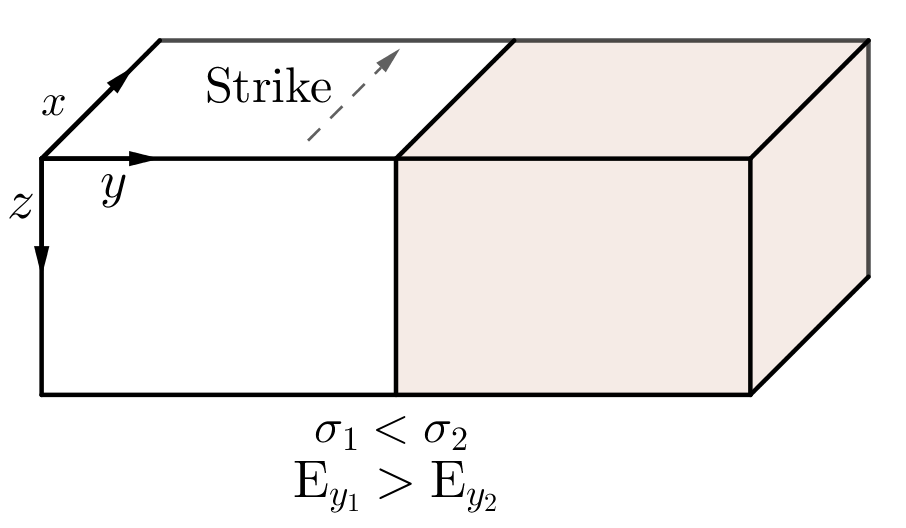
\includegraphics[width=10cm]{texto/fig/Tm_Te.png} 
	        \end{center}
		\fonte{Adaptado \cite{didana2010}}
		\label{fig_strike}
	    \end{figure}
	    
	    
	    
	    
	    Devido a essa diferença entre as resistividades elétricas polarizamos os campos em TE (Transversal Elétrico) e TM (Transversal Magnético).
	    Para esse modelo temos o tensor impedância como:
	    \begin{equation}
	     \textrm{Z}_{2D} = \left (\begin{array}{cc}
	                               0 & \textrm{Z}_{xy} \\
	                               \textrm{Z}_{yx} & 0
	                              \end{array} \right)
	    \end{equation}
	    Assim cada polarização pode ser escrita como:
	    \begin{equation}
	     \textrm{TE} = \left \{ \begin{array}{l}
	            \dfrac{\partial \textrm{E}_x}{\partial y} = \dfrac{\partial \textrm{B}_z}{\partial t} = -i\omega \textrm{B}_z \\[10pt]
	           \dfrac{\partial \textrm{E}_x}{\partial z} = \dfrac{\partial \textrm{B}_y}{\partial t} = i\omega \textrm{B}_y \\[10pt]
	           \dfrac{\partial \textrm{B}_z}{\partial y} - \dfrac{\partial \textrm{B}_y}{\partial z} = \mu \sigma \textrm{E}_x 
	           \end{array} \right.
	    \end{equation}
	    \begin{equation}
	     \textrm{TM} = \left \{ \begin{array}{l}
	            \dfrac{\partial \textrm{B}_x}{\partial y} = \mu \sigma \textrm{E}_z \\[10pt]
	           -\dfrac{\partial \textrm{B}_x}{\partial z} = \mu \sigma \textrm{E}_y \\[10pt]
	           \dfrac{\partial \textrm{E}_z}{\partial y} - \dfrac{\partial \textrm{E}_y}{\partial z} = i \omega \textrm{B}_x 
	           \end{array} \right.
	    \end{equation}
        
        
        \subsection{Terra 3D}
        Na maioria das condições geológicas o modelo se comporta como 3D, isso implica que a 
	    condutividade elétrica varia ao longo das três direções ($\sigma = \sigma_{x,y,z}$).
	    
	    A matriz do tensor impedância é então calculada com todos os termos. 
	    
	     \begin{equation}
	     \textrm{Z}_{3D} = \left (\begin{array}{cc}
	                               \textrm{Z}_{xx} & \textrm{Z}_{xy} \\
	                               \textrm{Z}_{yx} & \textrm{Z}_{yy}
	                              \end{array} \right)
	    \end{equation}

%=======================================================================================================================================================	    
    \chapter{\en{Softwares} Utilizados em Dados MT}
        \label{cap-proc_mt}
            
        Neste capítulo será discutido e mostrado como vinham sendo processados os dados \MT desde a etapa de coleta dos dados, até a produção de pseudo-secções. 
        
        Os programas utilizados são disponibilizados pelo \en{site} \citeauthor{mtnet}, \citeyearpar{mtnet}. O \en{site} MTnet é uma comunidade que une diversos programas para processamento de dados MT, para fins acadêmicos  
        
    \section{Aquisição de Dados MT}
        \label{sec_aquisicao_dados}
        O MT utiliza as frequências das ondas, isolando-as para obter um valor de resistividade, essas variam entre 1 $mHz$ e 10 $kHz$\footnote{Para aquisição Banda Larga} dentro do espectro eletromagnético.
        
        A escolha da taxa de aquisição dos dados é um fator importante, pois há um grande intervalo de períodos. Por exemplo, a frequência de 1 $mHz$ tem o período equivalente a 1000 $s$, ou seja, leva cerca de 17 minutos para que seja registrado um comprimento de onda em contra partida para 10 $kHz$ leva apenas 1 milissegundo.
        
        Para que seja contornada a problemática da aquisição são realizadas varias tomadas chamadas de bandas e cada uma é configurada com uma taxa de aquisição diferente, a tabela \ref{tab_taxa_aquisicao} mostra as taxas de aquisições frequentemente usadas. 
        
        \begin{table}[H]
                \centering
                \caption{Taxas de Aquisições frequentemente usadas para equipamentos ADU06 e ADU07.}
                \label{tab_taxa_aquisicao}
                \resizebox{0.5\textwidth}{!}{%
                \begin{tabular}{@{}ccc@{}}
                    \toprule
                    \textbf{Equipamento}  & \textbf{Banda}   & \textbf{Taxa de Aquisição [$H_z$]}   \\
                    \midrule
                                  &   A       &   65536     \\
                                  &   B       &   4096      \\
                          ADU06   &   F       &   Livre     \\
                                  &   C       &   64        \\
                                  &   D       &   2         \\
                                  &   65536H  &   65536     \\
                          ADU07   &   4096H   &   4096      \\
                                  &   128H    &   128       \\
                                  &   4H      &   4         \\
                    \bottomrule
                \end{tabular}%
                }
                \fonte{O Autor, 2018}
            \end{table}
        
        Como discutido na subsecção \ref{subsec-Impedancia} para se obter a matriz impedância é necessário efetuar a aquisição das componentes dos campos elétricos e magnéticos separadamente.
        
        Essas componentes são registradas em $[mV/Km]$ e em $[nT]$ para os campos elétricos e magnéticos respectivamente e são chamadas de séries temporais. As cinco séries temporais ($\textrm{E}_x,\, \textrm{E}_y, \, \textrm{H}_x, \, \textrm{H}_y \, \, \textrm{e} \, \, \textrm{H}_z$) são armazenadas em um arquivo binário com extensão padrão TS.
        
        \begin{figure}[H]
            \centering
	        \caption{Series Temporais das cinco componentes contidas no arquivo TS}
	        \begin{center}
	        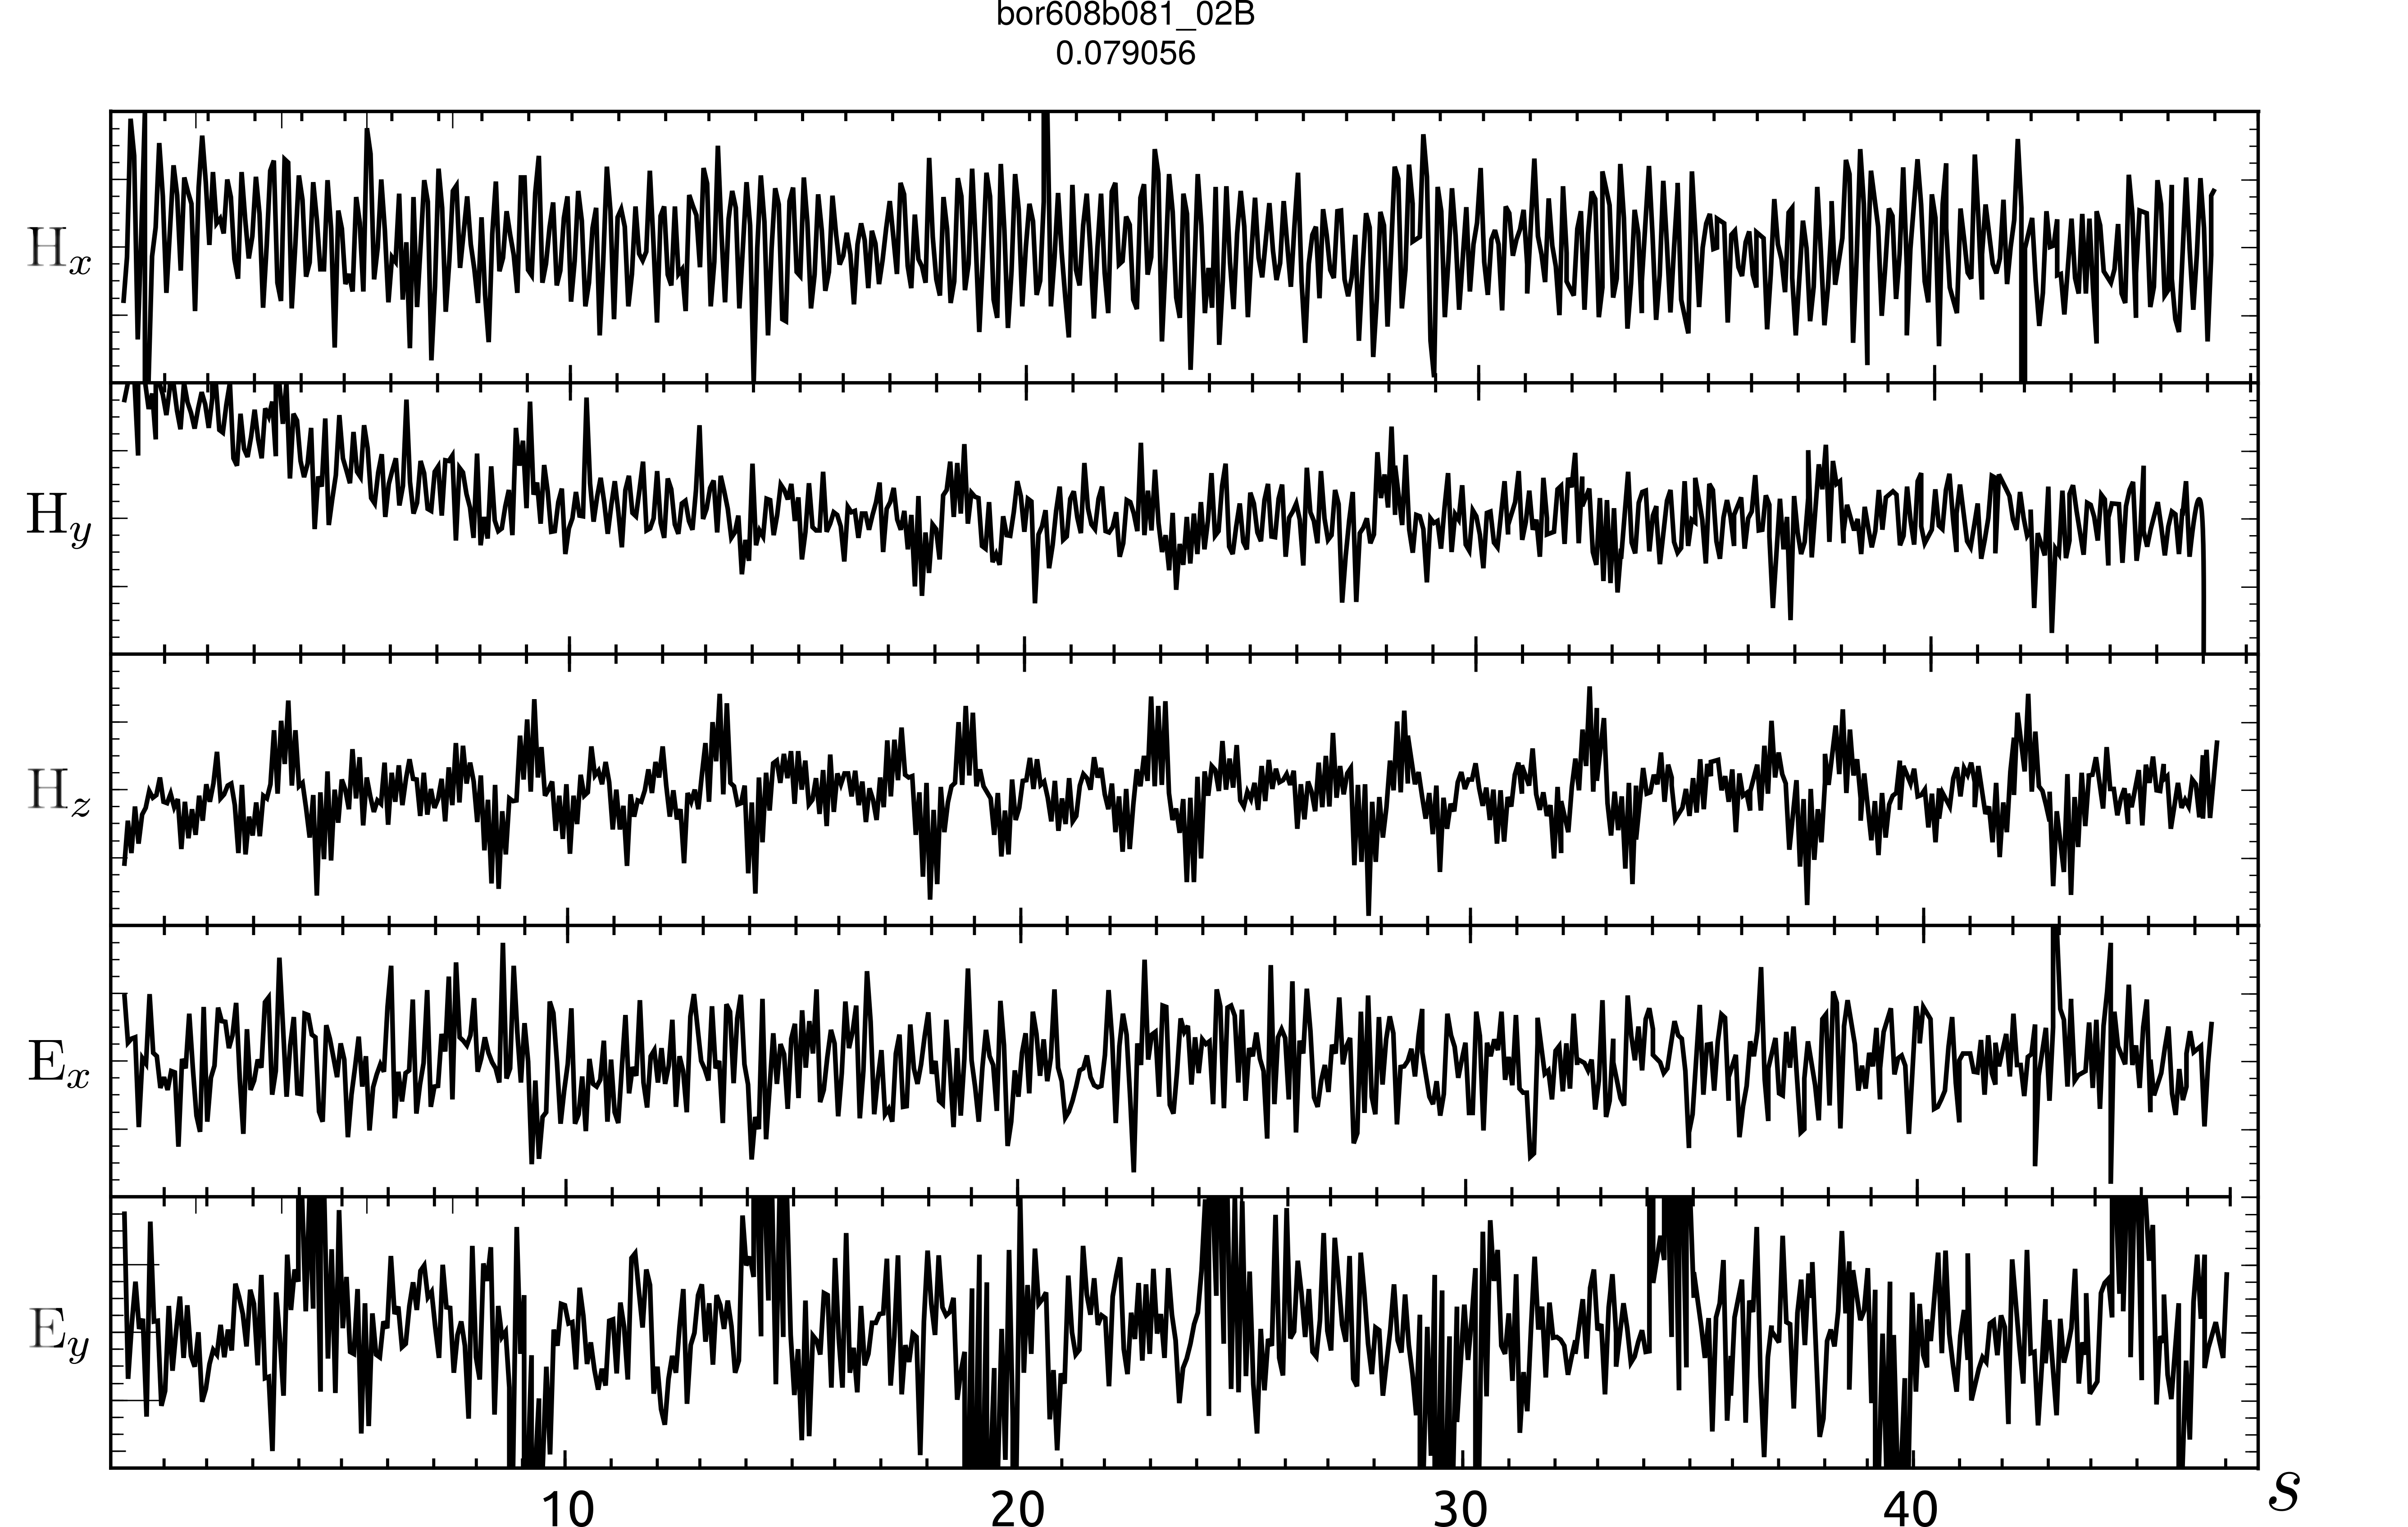
\includegraphics[width=13cm]{texto/fig/campos_divididos.png} 
	        \end{center}
		\fonte{O Autor, 2018}
	    \end{figure}
        
        \subsection{Estrutura do Aquivo TS}
            \label{subsec-arquivoTS}    
            Os arquivos .TS (\en{Time Series}) são arquivos binários e estruturados em 3 blocos; comentários, informações e dados  \cite{tsformat}.
            \begin{itemize}
             \item O Bloco de comentários é marcado pelo símbolo \en{\#} e todas essas linhas serão ignoradas pelo programa.
             \item   O Bloco de informações contém todas as propriedades da aquisição, como: coordenadas, elevação, declinação magnética, nome da estação, dentre outras.
             \item O bloco de dados contém 5 colunas e cada valor sendo igual ao registrado pelos sensores, a sequência das colunas são: $\textrm{H}_x,\, \textrm{H}_y, \, \textrm{H}_z, \, \textrm{E}_x \, \, \textrm{e} \, \, \textrm{E}_y$.
            \end{itemize}

    
    \section{Fluxo de Processamento de Dados MT}
       
        Como visto anteriormente (subsecção \ref{subsec-Impedancia}) a matriz impedância é obtida através das componentes $\textrm{H}_x,\, \textrm{H}_y,  \, \textrm{E}_x \, \, \textrm{e} \, \, \textrm{E}_y$. Porém as mesmas devem estar no domínio da frequência angular, discutido na secção \ref{sec_aquisicao_dados}. As séries temporais são obtidas com taxas de aquisições diferentes, isso implica que o tempo de leitura também será diferente, esse fato propicia que sejam feitas várias leituras com mesma taxa no mesmo ponto, essas leituras são chamas de rodadas. 
        
        O pré-processamento compreende essas etapas: converter os dados de binários para ASCII, para que possam ser manipulados facilmente; utilizar a transformada de Fourier para mudar o domínio dos dados de tempo para frequência angular; filtrar e escolher as melhores rodadas, ou seja, as séries que tiverem a maior coerência e menor ruído.
        
        A figura \ref{fig_fluxo_classico} ilustra todas as etapas de pré-processamento e as subsecções a seguir mostra quais os programas utilizados atualmente e como eles atuam sobre os dados.  
    
        
    \begin{figure}[H]
                \caption{Fluxograma de Processamento Clássico}
                \begin{center}
                    
\includegraphics[width=16cm]{texto/fig/fluxograma.png} \end{center}
                \fonte{O Autor, 2018}
                \label{fig_fluxo_classico} 
            \end{figure}
 
    \subsection{Conversão de Dados Binários}
    \label{subsec-conver-dados}
    Os arquivos TS são Binários não formatados, sendo que cada linha do arquivo é composta por 80 carácteres. 
    
    O comando \verb|ats2asc| \cite{emtf} é usado para a conversão dos dados, ele efetua a leitura do arquivo, a conversão para ASCII e a separação do arquivo em diferentes diretórios.
    
    A separação do arquivo é dada pela seguinte forma:
    
    \begin{enumerate}
     \item Diretório DATA/ 
     \subitem Arquivos asc $\rightarrow$ Contém as leituras dos sensores.
     \subitem Arquivos clk $\rightarrow$ Contém a hora que foi iniciada a rodada e também a hora de uma estação para referência remota.
     \item Diretório SP/
     \subitem Aquivos sp $\rightarrow$ Contém os parâmetros da aquisição.
    \end{enumerate}

    %Sintaxe do comando \verb|ats2asc|:
    %\begin{quote}
    % \codbox{ ats2asc \f{-{}-site-name} name\_site \cl{PATH\_site} 
    %        } \codnum{\ref{subsec-conver-dados}.1}
    %\end{quote}
    
    \subsection{Dnff}
    
            O programa Dnff faz parte do pacote EMTF \cite{emtf} desenvolvido por Gary D. Egbert, o pacote EMTF compõem rotinas de mudança de domínio dos dados e processamentos estatísticos para remoção de ruídos.
            
            O Dnff é responsável por fazer a transformada discreta de Fourier sobre os dados e aplica os coeficientes de Fourier que ajustam os problemas de reverberação.

    \subsection{TranMT}
    
            O programa TranMT também faz parte do pacote EMTF e é responsável por fazer os tratamentos estáticos sobre o dado, removendo \en{outliers} (pontos muito distantes da curva de tendência) e aumentar a relação sinal/ruído.
            
            A saída do programa TranMT são arquivos ZSS (formato padrão adotado por Egbert) contendo os valores de impedância e fase para cada janela. As janelas são como taxas de aquisições dentro dos arquivos obtidos em campo, essas podem ser configuradas pelo usuário ajustando a melhor representação dos dados em função da taxa de amostragem de aquisição em campo.   
            
            
    \subsection{ToJones}
    
            O programa Tojones \cite{tojones} extrai as informações dos arquivos ZSS de diferentes janelas e mescla os mesmo em um único arquivo J-format, onde, esses arquivos são usados para plotar as pseudo-secções e outras rotinas como o Rho+ \cite{rhoplus} e programas de inversão.
            
    \section{Pacotes de Processamentos do grupo Geoma - INPE}
    
        O grupo Geoma do INPE (Institudo Nacional de Pesquisas Espaciais) oferece um treinamento para processamento do \MT para alunos e colaboradores.
        
        Os \en{scripts} oferecidos para o processamento MT foram desenvolvidos pelo Dr. Marcelo Banik de Pádua obtidos sobre comunicação privada pelo autor.
        
        A natureza dos pacotes são \en{scripts} escritos em \en{Shell}, \en{Python}, \en{C++} que utilizam o programa GMT \cite{gmt} para plotagem dos gráficos.
        
        Os \en{script} auxiliam na utilização dos programas já citados, visto que a saída de um programa é a entrada do próximo. Um exemplo é o programa processamentoZ que prepara os dados para as rotinas Dnff e TranMT, ele ajusta os parâmetros necessários para esses programas e trabalha com os dados de forma padrão auxiliando o usuário na utilização dos pacotes. 
        
       
    
    

    
    
%========================================================================================================================================================    
    \chapter{Proposta de \en{Software} Livre Integrador}
    
        O desenvolvimento do \textit{software}, chamado de PampaMT, foi baseado na filosofia de \textit{Software Livre} \cite{soft_free} onde o código fonte será liberado e distribuído para a comunidade geofísica. A linguagem base escolhida para o projeto foi o Python, visto as vastas bibliotecas para trabalhar com dados científicos e a simplicidade da implementação do código.  
        
        \section{Linguagem PYTHON}
            \label{lim_python}
            
            Criada nos anos 80 por Guido Van Rossum no CWI (\en{Centrum Wishunde \& Informatica}) em Amsterdã, Holanda a linguagem Python foi idealizada no grupo de desenvolvimento da linguagem ABC do CWI, onde rapidamente começou a se destacar.
            
            Na década de 90 foi criada a \en{Python Software Activity} que começou a cuidar dos interesses da linguagem, nesse período apenas o criador Guido Van tomava as decisões e cuidava do desenvolvimento. Finalmente em 2001 é fundada a \en{Python Software Foundation} que mantém a linguagem e todos os direitos sobre ela \cite{python36}.  
            
            Python é uma linguagem de alto nível\footnote{Está relacionada a abstração da linguagem, alto nível significa mais longe da linguagem de código de máquina} onde seu código deve ser organizado favorecendo a interpretação e sendo ao mesmo tempo simples.
            
            Exemplos de código Python:

            Mostrar conteúdo na Tela:
            
            Como comentado, o código tem fácil leitura. Para imprimir um conteúdo na tela, por exemplo, 
            podemos simplesmente usar o comando \verb|print|, aproximando muito da língua inglesa.  
            \begin{quote}
             \codbox{\ini   \cc{Comentários}                  \\
                     \ini   \f{print} ('Hello World')         \\
                     Hello World
                     }                                          \codnum{\ref{lim_python}.1}

            \end{quote}
            
            Operações Matemáticas:
            
            As variáveis no código não precisam ser declaradas para um 
            tipo específico (Ex.: \textit{float, int, string}), como em outras linguagens, o que deixa o código mais fluido. 
            \begin{quote}
            
             \codbox{\ini a = 2                               \\
                     \ini b = 5                               \\
                     \ini \f{print}(a + b)                    \\
                     7                                        \\
                     %\ini                                    \\
                     \ini \f{print}(b / a)                    \\
                     2.5                                      \\
                     %\ini \cl{class} Tela(App):              \\
                     %\init  \cl{return} Tela
                     }                                          \codnum{\ref{lim_python}.2}
            \end{quote}
            
            Importando Módulos:
            
            Módulos são estruturas que podemos importar objetos de um código a outro,
            no script \ref{lim_python}.3 importamos o valor de $\pi$ que esta contido na variável \verb|pi| dentro do pacote \verb|math|. 
            
            \begin{quote}
             \codbox{\ini \cl{import} math                    \\
                     \ini                                     \\
                     \ini pi = math.pi                        \\
                     \ini \f{print}(pi)                       \\
                     3.141592653589793
                    }                                           \codnum{\ref{lim_python}.3}
            \end{quote}
            
        \section{Módulos e Pacotes}
            
            A vasta quantidade de pacotes de terceiros para Python é o que faz a linguagem tão rica.
            De fato, os 
            pacotes facilitam a implementação do código, por exemplo, se for preciso calcular o espectro de 
            frequência de um conjunto de dados, não será necessário implementar todo o algoritmo para efetuar o cálculo, resolver as integrais e assim por diante, mas sim podemos utilizar o pacote \verb|scipy| e importarmos a função \verb|fftpack| que já foi implementada e executar em nosso código, esse processo economiza tempo em desenvolvimento.           
            
            \subsection{Kivy}
            
            
            \label{lim_kivy}
            Kivy é um \textit{framework} criado em 2010 pela KIVY ORGANIZATION \cite{kivy} e \textit{Open Source} para o desenvolvimento de interfaces gráficas, a escolha dessa interface foi a alta compatibilidade entre sistemas operacionais e todo o processamento nativo para desenhar a tela é feita no chip gráfico liberando então mais processamento pela CPU.
            
            Kivy também é uma linguagem de programação que permite a criação da interface de forma mais fácil, similar ao QT \cite{qt} ela usa uma linguagem de marcação e indentada onde as propriedades dos \textit{widgets} (Objetos interativos com o usuário) são adicionadas colocando-as a baixo e com espaçamento de 4 espaços do \textit{widget}. 
                        
            Exemplo do Kivy dentro do código Python:
            \begin{quote}
             \codbox{\ini \cl{from} kivy.app \cl{import} App                      \\
                     \ini \cl{from} kivy.uix.button \cl{import} Button            \\
                     \ini                                                         \\
                     \ini      \cl{class} Test(App):                              \\
                     \init          \cl{def} build(self):                         \\
                     \init \,\,\,\,\,\,     \cl{return} Button(\ob{text}=\st{'Hello World')} \\
                     \ini                                                         \\
                     \ini Test().run()                                            
             }                                                                    \codnum{\ref{lim_kivy}.1}
            \end{quote}
            
            \begin{figure}[H]
                \caption{Exemplo de janela com Kivy implementada somente com código Python}
                \begin{center}
                    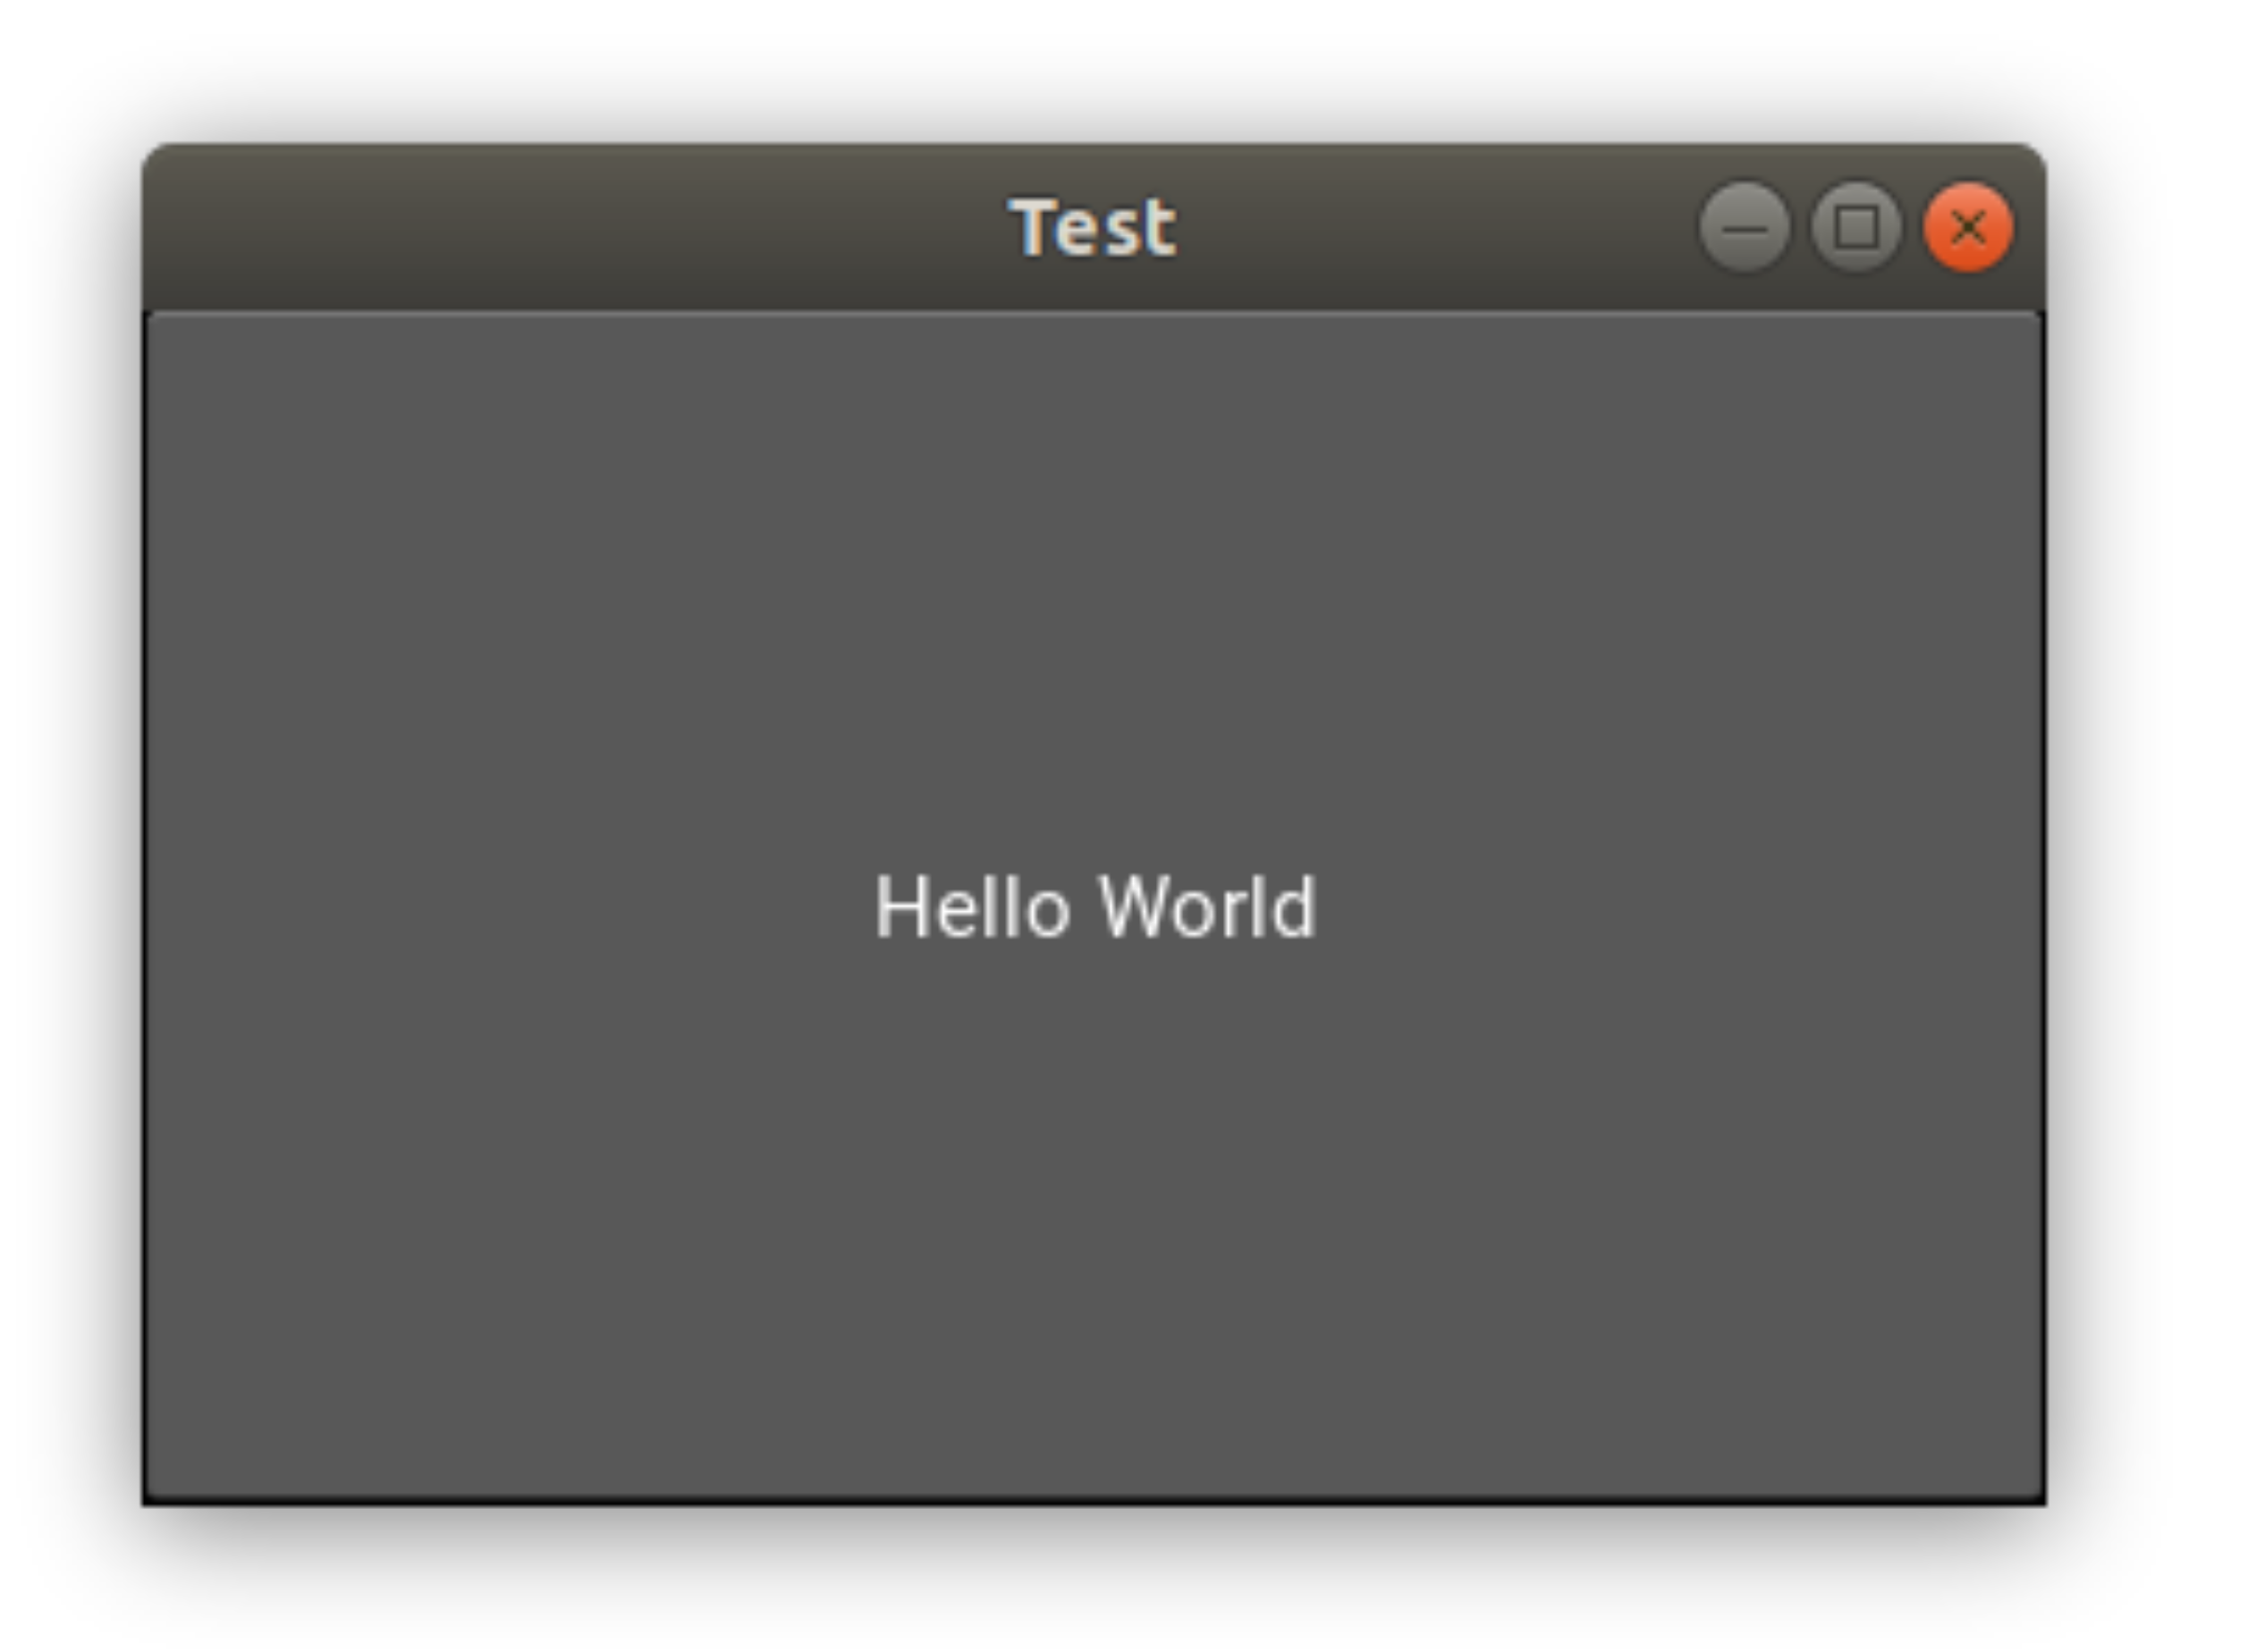
\includegraphics[width=7cm]{texto/fig/hello_world_kivy.png} 
                \end{center}
                \fonte{O Autor, 2018}
                \label{janela_kivy} 
            \end{figure}


            
            \subsection{SciPy, MatPlotLib, NumPy}
            \label{lim_scipy}
            
            SciPy é um ecossistema de ferramentas para processamento de dados científicos contando com ferramentes de manipulação de matrizes, plotagem de gráficos, interpolação dentro outras ferramentas \cite{scipy}.
            
            O ecossistema é de código aberto e as principais ferramentas são: NumPy para trabalhos com vetores e matrizes, MatPlotLib são ferramentas para plotagem de dados e o próprio SciPy para interpolação, cálculo de espectro de frequência dentre outras.
            
            A tabela \ref{pontos_ex_inter} apresenta 9 pontos distribuídos numa matriz quadrada de ordem 3, onde, a posição (2,2) possui uma anomalia, o código \ref{lim_scipy}.1 mostra como fazer a interpolação dos pontos e como plotar o resultado (figura \ref{fig_ex_inter}).
            
            \begin{table}[H]
                \centering
                \caption{Distribuição de pontos com valor anômalo ao centro.}
                \label{pontos_ex_inter}
                \resizebox{.22\textwidth}{!}{%
                \begin{tabular}{@{}cccl@{}}
                    \toprule
                    \textbf{Pontos}  & \textbf{x}   & \textbf{y}   & \textbf{z}  \\
                    \midrule
                        1&1       &   1     &  1     \\
                        %\hline
                        2&2       &   1     &  1     \\
                        %\hline
                        3&3       &   1     &  1     \\
                        %\hline
                        4&1       &   2     &  1     \\
                        %\hline
                        5&2       &   2     &  3     \\
                        %\hline
                        6&3       &   2     &  1     \\
                        %\hline
                        7&1       &   3     &  1     \\
                        %\hline
                        8&2       &   3     &  1     \\
                        %\hline
                        9&3       &   3     &  1     \\
                    \bottomrule
                \end{tabular}%
                }
                \fonte{O Autor, 2018}
            \end{table}
            

            Exemplo Numpy:
            \begin{quote}
             \codbox{\ini \cl{import} Numpy \cl{as} np        \\
                     \ini                                     \\
                     \ini  x = np.array([1,2,3,1,2,3,1,2,3])  \\
                     \ini  y = np.array([1,1,1,2,2,2,3,3,3])  \\
                     \ini  z = np.array([1,1,1,1,3,1,1,1,1])                                                                  
             }                                            \codnum{\ref{lim_scipy}.1}
            \end{quote}
            
            Exemplo SciPy:
            
            \begin{quote}
             \codbox{\ini \cl{from} scipy \cl{import} interpolate              \\
                     \ini \cl{from} scipy.interpolate \cl{import} griddata     \\
                     \ini                                                      \\
                     \ini  xi = np.arange(x.min(), x.max(), .01)               \\
                     \ini  yi = np.arange(y.min(), y.max(), .01)               \\
                     \ini  xi,yi = meshgrid(xi,yi)                             \\
                     \ini                                                      \\
                     \ini  \cc{ Interpolate}                                   \\
                     \ini  zi = griddata((x,y),z,(xi,yi),\ob{method}=\st{'cubic'})       
             }                                                                    \codnum{cont. \ref{lim_scipy}.1}
            \end{quote}
            
            Exemplo Matplotlib:
            
            \begin{quote}
             \codbox{\ini \cl{import} matplotlib.pyplot \cl{as} plt            \\
                     \ini                                                      \\
                     \ini  plt.figure(1)                                       \\
                     \ini  plt.subplot(111)                                    \\
                     \ini                                                      \\
                     \ini  zn = np.arange(z.min(), z.max() + 0.01, .01)        \\
                     \ini                                                      \\
                     \ini  plt.plot(x, y, \st{'kx'})                           \\
                     \ini  plt.contourf(xi, yi, zi, zn)                        \\
                     \ini  plt.colorbar()                                      \\ 
                     \ini  plt.grid()                                          \\
                     \ini  plt.set\_cmap(\st{'jet'})                           \\
                     \ini  plt.show()                                          \\
             }                                                                   \codnum{cont. \ref{lim_scipy}.1}
            \end{quote}
            
            \begin{figure}[H]
                \caption{Exemplo dos pontos interpolados usando SciPy e plotados usando MatPlotLib}
                \begin{center}
                    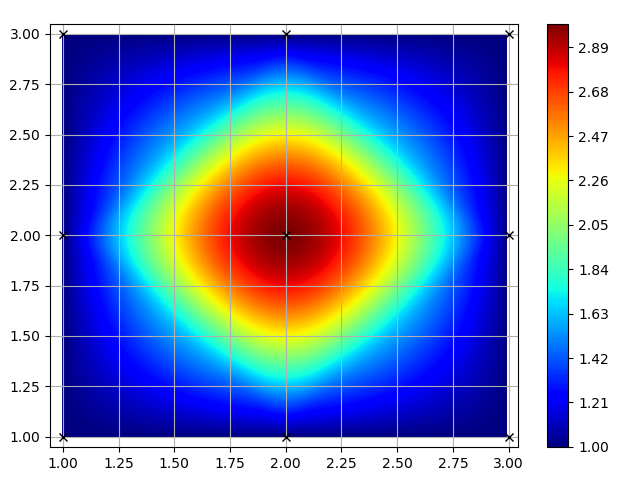
\includegraphics[width=9cm]{texto/fig/plot_ex.png} 
                \end{center}
                \fonte{O Autor, 2018}
                \label{fig_ex_inter} 
            \end{figure}
    
    \section{Arquitetura do Programa e Abordagem dos fluxos de Processamento}
        \label{cap-algoritmos}
    
    
    O PampaMT trabalhará com os dados seguindo os fluxos de processamentos comentado no capitulo \ref{cap-proc_mt}, atualmente o maior consumo de tempo de processamento são destinados a essas etapas. O programa desenvolvido focará em melhorar o tempo de processamento, visualização dos dados e aprendizagem.
    
    O fluxograma da figura \ref{fig_influ_mainpy} ilustra as etapas de inicialização pensados para o programa e como será a execução do pacote EMTF sobre os dados.
    
    Como já discutido as etapas de processamento serão feitas através de interface gráfica e o programa processamentoZ será reescrito para aumentar a compatibilidade no fluxo.
    
    O fluxograma da figura \ref{fig_influ_pampamtpy} mostra o processo principal do programa, onde o usuário poderá:
    \begin{enumerate}
     \item Plotar as janelas
     \item Escolher os períodos para cada janela
     \item Executar o processamentoZ para novas rodadas
     \item Executar o Tojones sobre as janelas escolhidas
    \end{enumerate}

    Após o Tojones é finalizado o processo, compreendendo então todas as etapas propostas no trabalho.
    
  
    
    
    
    \begin{figure}[H]
                \caption{Fluxograma Tela Principal PampaMT}
                \begin{center}
                    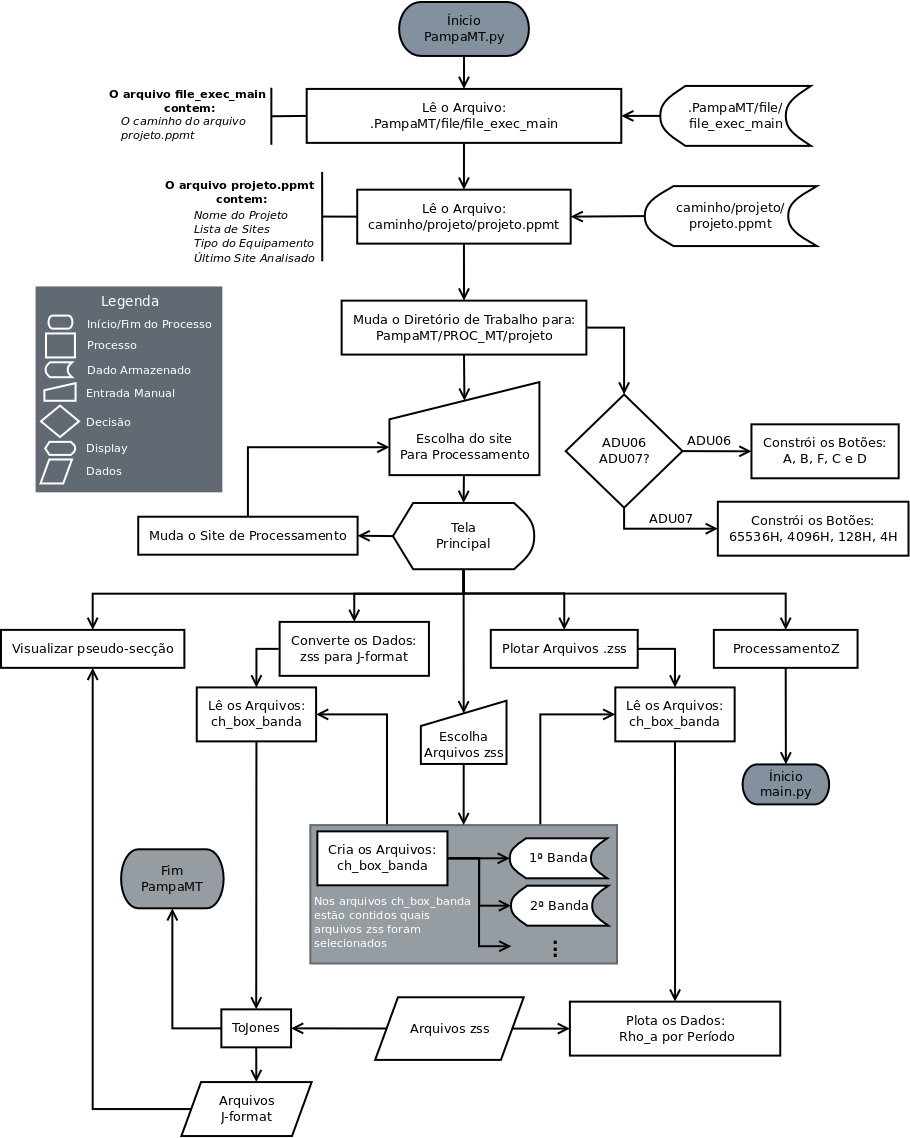
\includegraphics[width=15cm]{texto/fig/PampaMTpy2.png} 
                \end{center}
                \fonte{O Autor, 2018}
                \label{fig_influ_pampamtpy} 
            \end{figure}
            
            
    \begin{landscape}
    
    \begin{figure}[H]
                \caption{Fluxograma de Inicialização do PampaMT}
                \begin{center}
                    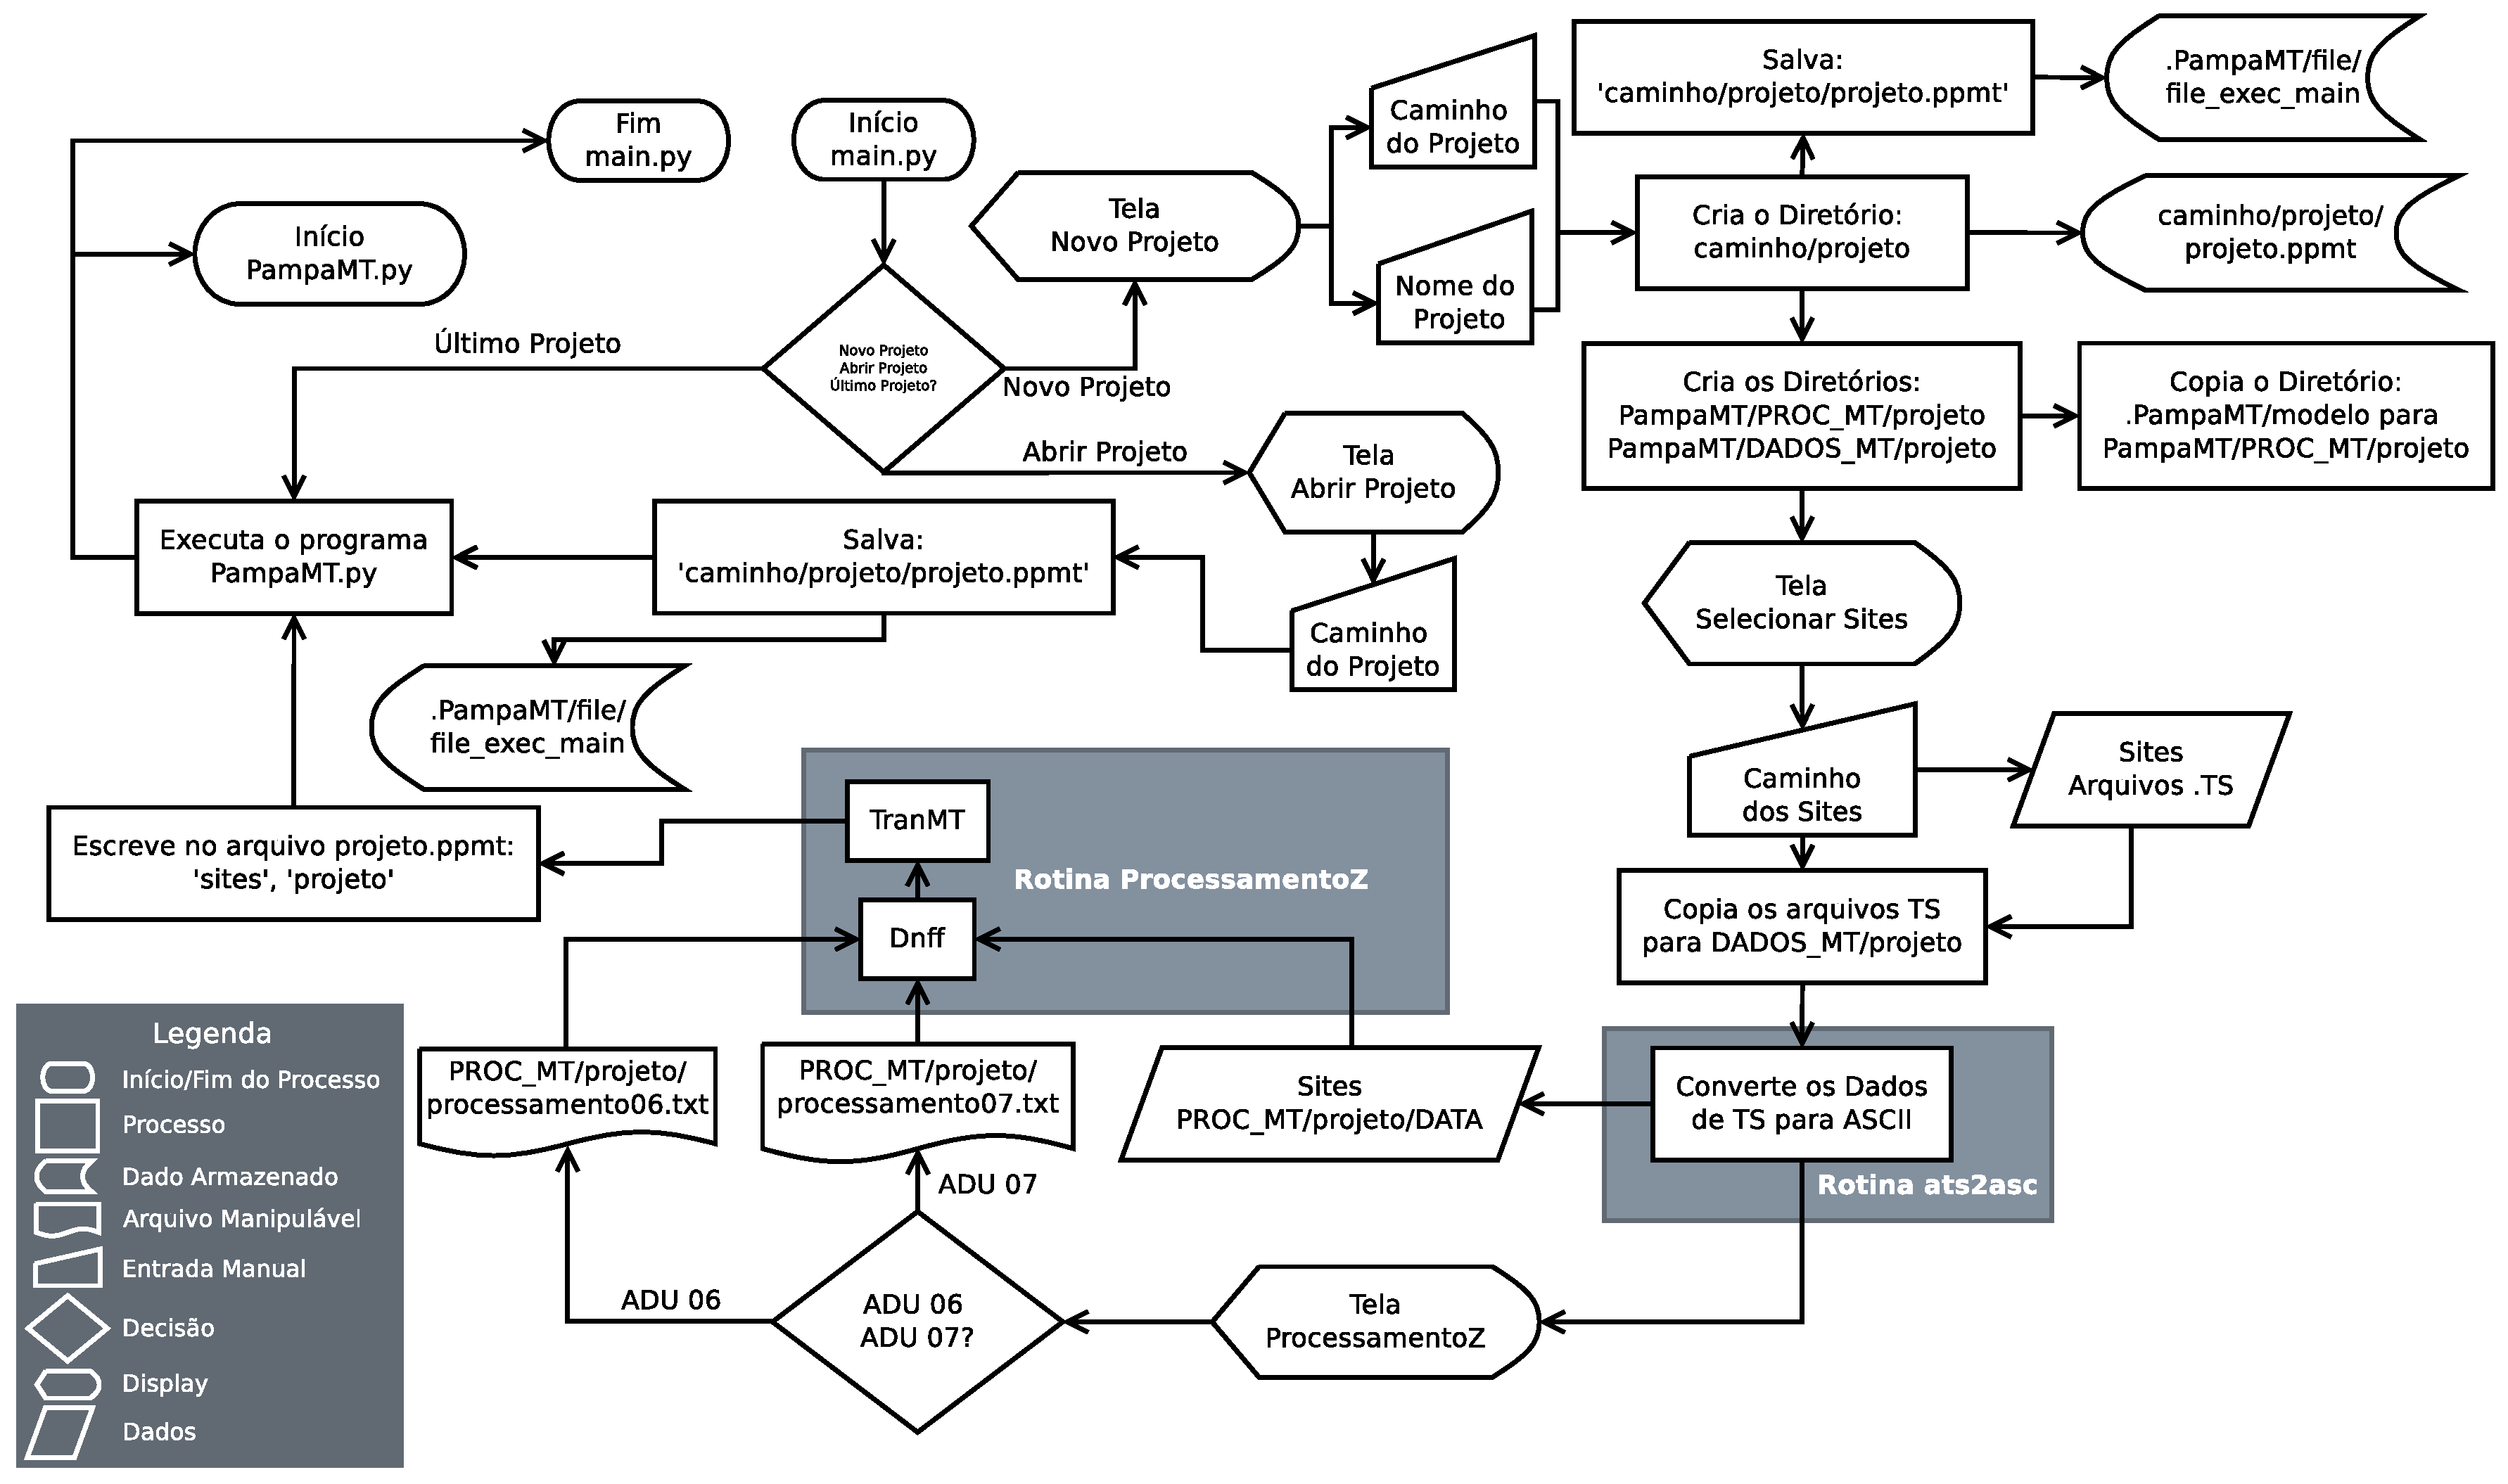
\includegraphics[width=21cm]{texto/fig/mainpy.eps} 
                \end{center}
                \fonte{O Autor, 2018}
                \label{fig_influ_mainpy} 
            \end{figure}
    \end{landscape} 
